\chapter{Introduction}
\label{Introduction}
\graphicspath{{Figures/Introduction/}{Figures/Common/}}

It is hard to underestimate the effect that the laser has had since its invention in 1960 \citep{Maiman:1960}.  Although initially motivated by pure scientific curiosity, its unique properties have given it application in an astonishing array of technologies, in addition to its use as a powerful tool in fundamental research.  

Laser radiation is distinguished from the light emitted by everyday light sources --- such as light bulbs --- by three main properties, (i) its narrow divergence, (ii) the narrow range of frequencies that are emitted, and (iii) the \emph{coherence} of the emitted radiation.  Although many applications only make use of the first two properties, the coherence of a laser is critical to its use in such applications as laser gyroscopes, gravitational wave detection and fundamental tests of quantum mechanics\footnote{FIXME: Add citations}.  Crudely, the coherence of light is related to the extent to which knowledge of its phase at one instant can be used to predict its phase at later times.  Light emitted from a light bulb is chaotic: its phase evolves randomly in time.  Light emitted from a laser is highly predictable: its phase evolves linearly in time with some phase diffusion over longer time scales.  

Quantum mechanics tells us that not only can light behave as a wave, but atoms can too.  This wave nature of atoms is usually indiscernible because the typical wavelength for a thermal atom is many orders of magnitude smaller than the inter-atomic spacing ($\lambda \sim 5 \times\unit[10^{-11}]{m}$ as compared to $d \sim 3 \times\unit[10^{-9}]{m}$).  However, in 1925 Einstein predicted \citep{Einstein:1925} that if a gas of \emph{bosons} (a class of particles which includes many atomic species) was cooled below a critical temperature, a large fraction of the particles would occupy the ground state of the system, forming a coherent wavefunction.  This was achieved in 1995 for dilute atomic gases \citep{Anderson:1995vn,Bradley:1995ys,Davis:1995} with the first production of a Bose-Einstein Condensate (BEC), a macroscopic occupation of atoms in a single spatial mode.  As it is the macroscopic occupation of \emph{photons} in a single spatial mode that gives the optical laser many of its properties, with the achievement of BEC it has become possible to consider the creation of an atomic analogue of the optical laser: the \emph{atom} laser.

An atom laser, while ideally sharing the above properties of its optical cousin, would behave very differently to an optical laser.  While photons interact strongly with matter, they interact only weakly with themselves or with gravity.  While this makes lasers robust to fluctuations in electromagnetic or gravitational fields, they are therefore less sensitive to these fields in interferometry experiments.  Despite this limitation, optical interferometry has been used in several incredible gravitational experiments, including GRACE, LIGO, and Gravity Probe-A \citep{Vessot:1980}.

Somewhere the award of the Nobel prizes for BEC and related work should be mentioned as it is a rapidly evolving, and exciting field of tremendous importance.  Or something.


it means that they are less sensitive to these effects in interferometry experiments where they are under investigation.  


amazing gravity experiments with lasers: GRACE, LIGO, eventually, LISA

they do not interact strongly with themselves or with gravity.  

It is the narrow spectral linewidth, the high spectral intensity, and its large coherence length that give the optical laser such a wide range of applications.  These properties themselves derive from the macroscopic occupation of photons in a single optical mode inside the laser cavity.  With the achievement of Bose-Einstein Condensate (BEC) in 1995 \citep{Anderson:1995vn,Bradley:1995ys,Davis:1995} --- a macroscopic occupation of \emph{atoms} in a single spatial mode --- there has arisen the experimental challenge of producing an atomic analogue of the optical laser: the \emph{atom} laser.  As atoms interact more readily with their environment than photons, atom interferometry has a broad range of applications: to the measurement of electric and magnetic fields in tests of atom and neutron charge neutrality \citep{Arvanitaki:2008}, an application which would be essentially impossible with optical lasers due to the weak photon--photon interaction; to fundamental tests of predictions of General Relativity \citep{Dimopoulos:2007uq}; to the development of gyroscopes \citep{Gustavson:1997}, gradiometers \citep{Snadden:1998,McGuirk:2002} and gravimeters \citep{Peters:2001}, which, while possible using optical lasers, their atomic counterparts are far more compact due to the significantly stronger gravitational interaction.

more broadly and to the development of more compact sensors.  




Although the low kinetic energy of atom lasers would prevent their use 


The differences between an atom laser and an optical laser derive from the inherent differences between photons and atoms: atoms interact much more readily with their environment.  This is both a blessing and a curse.  It is a blessing

 over an optical laser derives from the 



First cw optical laser \citep{Javan:1961}.


The achievement of Bose-Einstein Condensate (BEC) in 1995 \citep{Anderson:1995vn,Bradley:1995ys,Davis:1995} has led to the possibility of creating an analogous source for atoms, which could take advantage of the inherent differences between photons and atoms.  Atoms interact much more readily with their environment, giving atom interferometry applications in fundamental tests of predictions of General Relativity \citep{Dimopoulos:2007uq}, tests of atom and neutron charge neutrality \citep{Arvanitaki:2008}, gyroscopes \citep{Gustavson:1997}, gradiometers \citep{Snadden:1998,McGuirk:2002} and gravimeters \citep{Peters:2001}.  FIXME: How many of these actually use atom lasers, and how many use thermal beams?

The increased interactivity of atoms over photons is both a blessing and a curse: while it is the source of crap.

far more sensitive to fluctuations in external electric or magnetic fields, etc


We need to talk about thermal beams, briefly.

Discussion of cold thermal atom interferometry, and how this can be improved through the use of atom lasers. 

Rotation sensing using cold thermal atom clouds: \citep{Canuel:2006}, measuring Newton's constant $G$: \citep{Lamporesi:2008}


Here goes the motivation.

Steal everything that we can from papers.

\section{Photon lasers and Atom lasers}
\label{Introduction:PhotonAndAtomLasers}

The basic features necessary of a continuous atom laser are analogous to the features of a continuous photon laser: a resonant, a lasing mode, an outcoupling process, and a Bose-stimulated pumping mechanism (see \figureref{Introduction:LaserAtomLaserComparison}).  The first three of these features are well understood for an atom laser; experimentally realising the fourth, the pumping mechanism, has presented the greatest challenge.

\begin{figure}
    \centering
    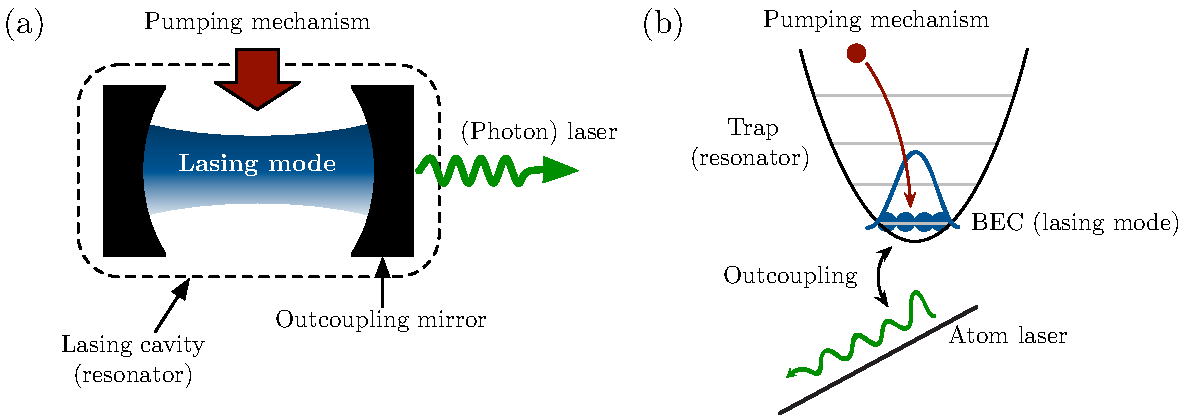
\includegraphics[width=14cm]{LaserAtomLaserComparison}
    \caption{
        \label{Introduction:LaserAtomLaserComparison}
        FIXME: This is not a caption.
    }
\end{figure}

\subsection{The resonator}

In a photon laser, the resonator is typically a cavity formed between two (or more) mirrors trapping the photons with a region of space; the optical mode trapped within the resonator is the lasing mode.  For atom laser, the resonator is an `atom trap', either an optical trap using the ac Stark shift to trap the atoms in a region of high optical intensity, or a magnetic trap using the Zeeman shift to selectively trap certain magnetic hyperfine states near a local minimum of the magnetic field.

\subsection{The lasing mode}

\begin{figure}
    \centering
    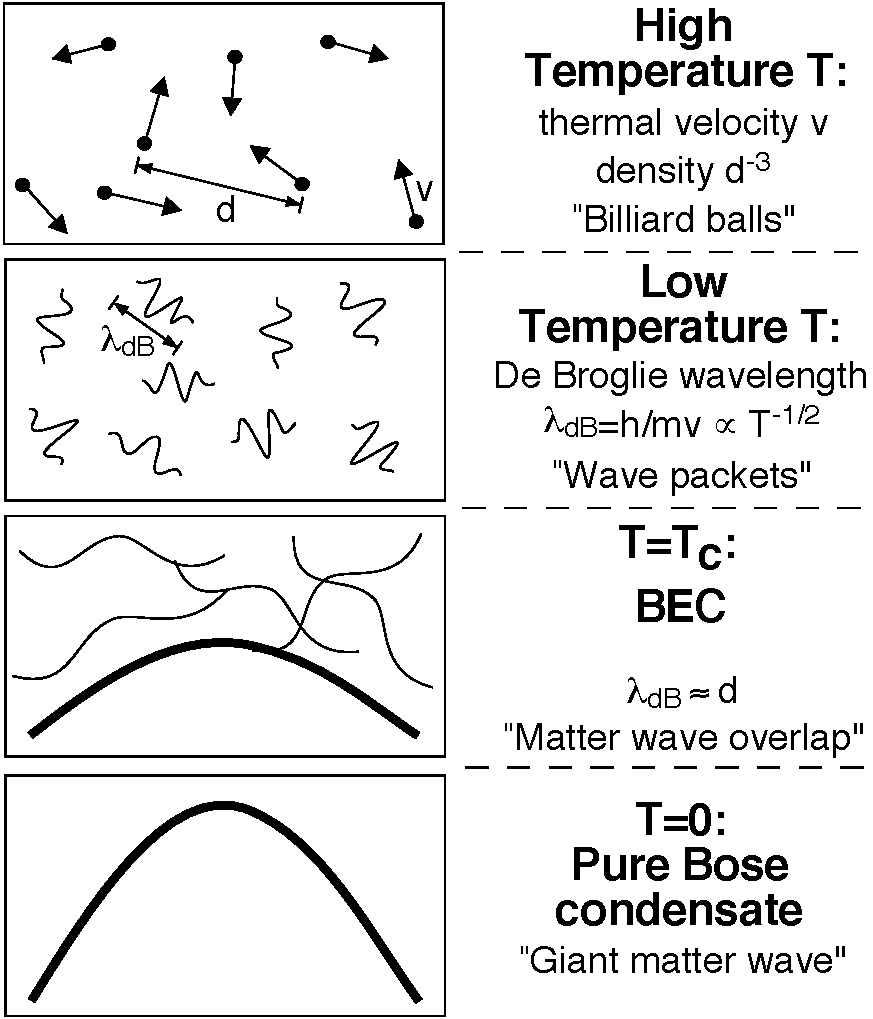
\includegraphics[width=8cm]{WhatIsBEC}
    \caption{
        \label{Introduction:WhatIsBEC}
        FIXME: This is not a caption.  Figure stolen without permission from \citep{Ketterle:1999fk}.
    }
\end{figure}

The necessary property for the lasing mode of a laser --- be it optical or atomic --- is that it have an occupation much greater than one \citep{Wiseman:1997ba}.  For photons, such a highly-degenerate mode was first achieved with the development of the photon laser itself \citep{Maiman:1960,Javan:1961}; a photon condensate cannot exist in equilibrium as total photon number is not conserved \citep{Muller:1986,Ketterle:1999fk}.  Total atom number is, however, conserved and Bose-Einstein condensation occurs below a critical temperature \citep{PethickSmith}.  Below this critical temperature, a significant fraction of the atoms in the system occupy a single spatial mode; exactly what is required of the lasing mode of an atom laser.

The process of Bose-Einstein condensation can be understood in a simplified picture in which the atoms are viewed as wave-packets with an extent of the order of the thermal de Broglie wavelength $\lambda_\text{dB} = (2 \pi \hbar^2 / M k_B T)^{1/2}$, where $M$ is the mass of the atom, $k_B$ is Boltzmann's constant, and $T$ is the temperature of the atoms.  At room temperature, the de Broglie wavelength is sufficiently small ($\sim 5\times\unit[10^{-11}]{m}$ for \nucl{4}{He} at $T=\unit[300]{K}$) that the atoms behave as point-like billiard balls (upper panel of \figureref{Introduction:WhatIsBEC}).  As the temperature decreases, the de Broglie wavelength increases (second panel of \figureref{Introduction:WhatIsBEC}).  As the temperature continues to decrease, the de Broglie wavelength approaches the mean interparticle separation $d$ and the atomic matter waves begin to overlap (third panel of \figureref{Introduction:WhatIsBEC}).  Below this temperature, a Bose-Einstein condensate begins to form, until at $T=0$, all atoms are in the condensate (lower panel of \figureref{Introduction:WhatIsBEC}).  Conservation of total number is necessary for BEC, as it is because of this that the interparticle separation $d$ remains constant as temperature is decreased (in a box of constant volume); for photons, as the temperature is decreased the total number of photons in the system decreases, increasing the mean interparticle separation $d$ faster than the photon wavelength increases.  Hence photon condensation cannot occur in equilibrium.

Bose-Einstein condensation is a macroscopic quantum phenomenon with a broad range of applications beyond the production of atom lasers.  Perhaps the most interesting of these are the development of \emph{quantum simulators} \citep{Lewenstein:2007,Buluta:2009}, experiments which directly realise theoretical condensed matter models, which where initially proposed as approximations to other systems.  For example, the Bose-Hubbard model \citep{Fisher:1989} of interacting bosons was realised by loading a BEC into an optical lattice.  By changing the depth of the optical lattice, the ratio of the tunnelling and interaction terms was be changed, permitting direct observation of the superfluid--Mott insulator transition \citep{Greiner:2002lr}.  Quantum simulators are possible for a variety of other systems, including Josephson junctions \citep{Levy:2007vn}, and reduced-dimensional systems such as the Tonks-Girardeau model of 1D hard core bosons \citep{Girardeau:1960,Lieb:1963,Paredes:2004}.  Dilute gas BECs have also been used in the direct observation of persistent currents in the form of vortices and vortex lattices \citep{Abo-Shaeer:2001}, the coherent control of optical information \citep{Ginsberg:2007fk}, and the observation of quantum optical effects in atoms such as the Hanbury-Brown-Twiss effect \citep{Jeltes:2007fk}, and four-wave mixing \citep{Deng:1999qy}.

% Theoretical things not included in the above list:
% realisation of an analogue to a magnetic monopole \citep{Pietila:2009}
% super-chemistry \citep{Heinzen:2000}: perform a chemical reaction in a controlled way, from a desired initial state to a desired final quantum state
% GR-analogues

% Other things not mentioned:
% Testing Bogoliubov's theory for excitations and the speed of sound (temperature dependence too)

One of the advantages of dilute gas BEC that gives these systems such a broad range of applications is the extraordinary degree to which these systems can be controlled and manipulated:  their effective dimensionality can be changed by changing the confining potential; the de Broglie wavelength is controllable over many orders of magnitude $\unit[1]{nm} \lesssim \lambda_\text{dB} \lesssim \unit[10]{\micro m}$; the sign and magnitude of interparticle interactions can be controlled \citep{Inouye:1998hy}, all the way from attractive interactions through to infinitely repulsive interactions, including the non-interacting limit; essentially `pure' potentials (minimal absorption) may be constructed in a range of forms including highly regular potentials such as harmonic or lattice potentials, and random potentials with controllable statistical properties.  Dilute gas BEC also has a range of available observational tools for probing the system including absorptive imaging, phase-contrast imaging, Bragg scattering, and ionisation in the case of metastable species\footnote{FIXME: Missing citations everywhere}.  

The goal of atom optics is to use the fundamental differences between atoms and photons in the application of the principles of laser optics to new fields of research.

\subsection{The outcoupling process}

The outcoupling of light from the lasing mode of a photon laser is achieved by making one of the cavity mirrors partially transmissive.  The emitted light is the output mode of the photon laser.  For atom lasers, an analogous technique can be used in optical traps by lowering the depth of the trap until some atoms can tunnel out of the trap with the assistance of gravity.  In magnetic traps, electromagnetic radiation is applied to transfer the atoms (either directly with radio-frequency radiation \citep{Mewes:1997,Bloch:1999mi}, or indirectly via a multi-photon Raman transition \citep{Moy:1997,Hagley:1999dz,Robins:2006fk}) into a magnetically-insensitive state in which they fall freely under gravity.  These outcoupled atoms form the atom laser beam.

Contemporary atom optics experiments operate in pulsed mode.  Without a pumping mechanism, the atom laser beam is limited by the size of the condensate.  Once all of the atoms in the BEC have been outcoupled, the atom laser beam stops.  This places a fundamental limit on the linewidth (related to the longitudinal velocity-spread) of the atomic pulse produced: the Fourier limit, proportional to the inverse of the outcoupling time \citep{Johnsson:2007}.  This limit can be made arbitrarily small (until the energy uncertainty in the BEC due to interatomic scattering becomes significant \cite{Johnsson:2007a}) at the expense of an arbitrarily low atom flux.  Practically however, this trade-off cannot be made because the signal-to-noise ratio for atom laser experiments depends critically on the atomic flux \citep{Dowling:1998}.  The only way to achieve a high-flux atom laser with a narrow linewidth is with a continuous pumping process, which has yet to be achieved experimentally. 

The outcoupling process for atom lasers displays a range of behaviour.  While intuitively one might expect that increasing the outcoupling strength would continuously increase the atom laser flux, this is only true up to a point.  In the limit of large outcoupling rates a bound state forms \citep{Jeffers:2000rr}, and the atom laser shuts down \citep{Robins:2004pz}.  

The outcoupling process also strongly affects the transverse profile of the atom laser.  Due to the mean-field repulsion the atoms experience as they leave the condensate, significant interference fringes are observed on the atom laser profile \citep{Busch:2002zr,Kohl:2005fk}.  These interference fringes complicate the spatial profile of the atom laser, making any atom interferometry experiment that relies upon separated beam paths more challenging.  The interference fringes on the transverse profile increase the sensitivity of the experiment to imperfections in the spatial overlap of the previously-separated beams when they are combined for detection.  These interference fringes may be reduced by outcoupling from the bottom of the condensate \citep{Riou:2006uq} or by giving the atoms a significant momentum kick as they leave the condensate \citep{Jeppesen:2008}.  The transverse profile of the atom laser is discussed in greater detail in \sectionref{BackgroundTheory:TransverseProfile}.

Even in the absence of a pumping process, atom lasers can be used for a variety of interesting experiments.  The correlation and counting statistics of an atom laser have been measured \citep{Ottl:2005}, an atom laser has been guided with optical waveguides \citep{Guerin:2006mz}, and a BEC has been probed using an atom laser outcoupled from a separate BEC \citep{Doring:2008}.  There have also been interesting theoretical proposals to produce non-classical atom laser states using the interatomic interaction of the atom laser \citep{Johnsson:2007b}, or by outcoupling with squeezed light \citep{Haine:2005}, and a related proposal to generate controllable atom--light entanglement \citep{Haine:2006}.

% Comparison of multistate and two-state atom laser output couplers \citep{Dugue:2007fk}
% Quasi-monomode guided atom laser \citep{Couvert:2008}
% 
% Quantum-noise limits to the atom-laser gyroscope \citep{Dowling:1998} --- Perhaps this should go earlier?
% 
% First experimental studies of the divergence of the atom laser \citep{Le-Coq:2001vn}.
% Reducing the linewidth via feedback: \citep{Wiseman:2001zr}
% Bragg diffraction of an atom laser by an optical standing wave \citep{Wu:2006fj}
% It is claimed that gravitational wave detectors based on matter-wave interferometers are no better than laser interferometers \citep{Roura:2006}.
% Comparison of multistate and two-state atom laser output couplers \citep{Dugue:2007fk}
% Observation of transverse interference fringes: \citep{Dall:2007}
% Coherent splitting of an atom laser beam: \citep{Dugue:2008}
% Theoretical tools for atom laser beam propagation: \citep{Riou:2008}
% Quasi-monomode guided atom laser \citep{Couvert:2008}
% Two-state Raman outcoupler \citep{Debs:2009}

\subsection{The pumping mechanism}

\subsubsection{The photon laser}

The pumping mechanism of a laser acts as an amplifier for the lasing mode.  It is what replenishes the losses of the lasing mode due to outcoupling, and any other loss processes.  Without a pumping mechanism, an optical laser is simply a leaky cavity emitting an exponentially-decreasing amount of light.  The linewidth of this emitted light is limited by the linewidth of the optical cavity.  The pumping mechanism for an optical laser not only permits continuous operation of the laser, it also narrows the linewidth of the laser in a process known as \emph{gain-narrowing}.  Gain-narrowing results from the saturation of the pumping process for large signals; no physical amplifier can amplify a signal indefinitely.  

\begin{figure}
    \centering
    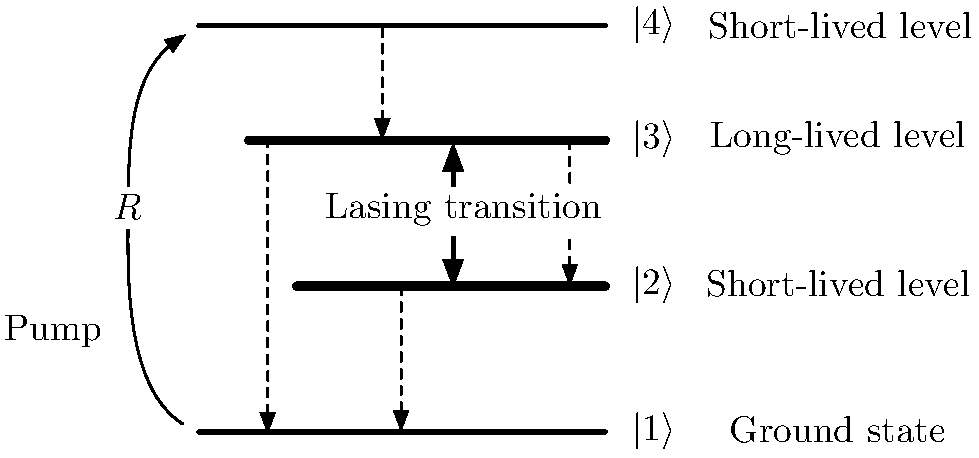
\includegraphics[width=10cm]{4LevelOpticalLaserModel}
    \caption{
        \label{Introduction:4LevelOpticalLaserModel}
        FIXME: This is not a caption.  Figure shamelessly plagiarised from Figure 13.2-6 of \citep{SalehTeich}.  Note that all levels have been incremented by 1 to avoid confusion with the vacuum state.  Figure needs clarifying, but can stand in for the present.
    }
\end{figure}

A pumping mechanism contains excitations that can each increase the occupation of the lasing mode by one.  These excitations are replenished at a finite rate, limiting the rate at which the lasing mode may be increased.  For example, in the 4-level photon laser model illustrated in \figureref{Introduction:4LevelOpticalLaserModel}, atoms are pumped from the ground state $\ket{1}$ to the short-lived state $\ket{4}$ at a rate $R$.  The atoms in state $\ket{4}$ may decay into the $\ket{3}$ state, the excited state of the lasing transition.  The occupation of the lasing mode can therefore not be increased at a rate greater than $R$.  Any physical pumping mechanism will also exhibit saturation, and therefore the laser mode will exhibit gain-narrowing.

Another necessary property of the pumping mechanism is that it be irreversible; once the occupation of the lasing mode has been increased, the probability that the process will reverse should be negligible.  This is achieved by coupling to a large number of essentially-empty modes known as a \emph{reservoir}.  In the case of the 4-level photon laser model depicted in \figureref{Introduction:4LevelOpticalLaserModel}, once an atom in the excited state of the lasing transition, $\ket{4}$ has undergone spontaneous emission into the $\ket{2}$ state, it rapidly decays into the ground state $\ket{1}$.  By ensuring that the ground state of the lasing transition $\ket{2}$ decays to the true ground state $\ket{0}$ faster than it can absorb a lasing photon, the pumping process is made irreversible.  The reservoir is comprised of the essentially-empty modes of the $\ket{2}$ level, which are kept empty due to their short lifetime.

Finally, in many circumstances it is desirable that the photon laser have only one lasing mode.  It is possible for a laser to support more than one lasing mode as the resonator may support many different modes, and if the gain bandwidth of the pumping mechanism encompasses more than one of these modes, multiple lasing modes may result.  As the photon--photon interaction is negligible, these lasing modes do not directly interact, and may operate independently.  Multiple-mode operation in a photon laser is naturally suppressed if the pumping process is \emph{homogeneously broadened}.  In homogeneously broadened gain media, every excitation of the pumping mechanism contributes to the gain of the lasing modes in the same way, i.e.\ every excitation has the same gain profile.  If the gain medium is \emph{inhomogeneously broadened}, some classes of pumping excitations will contribute differently to the total gain profile than others.  A classic example of this is Doppler-broadening.  Atoms in a gain medium will have a finite temperature, and their motion affects what frequencies they are resonant with in the laboratory frame due to the Doppler effect.  If the size of this frequency is greater than the natural width of the lasing transition, the saturation of those excitations resonant with one lasing mode may not affect the gain experienced by another lasing mode.  In this case, both lasing modes will experience gain independently, each without saturating the other.  If the pumping process is inhomogeneously broadened, undesirable modes can be removed by increasing their loss in the optical resonator.  This is naturally achieved by the addition of a second, smaller cavity inside the resonator that is only resonant with the desired mode.  If the pumping process is homogeneously broadened however, while multiple modes may initially experience gain, only the mode with the largest net gain will survive as the gain saturates, resulting in single-mode operation.


\subsubsection{The atom laser}

\begin{figure}
    \centering
    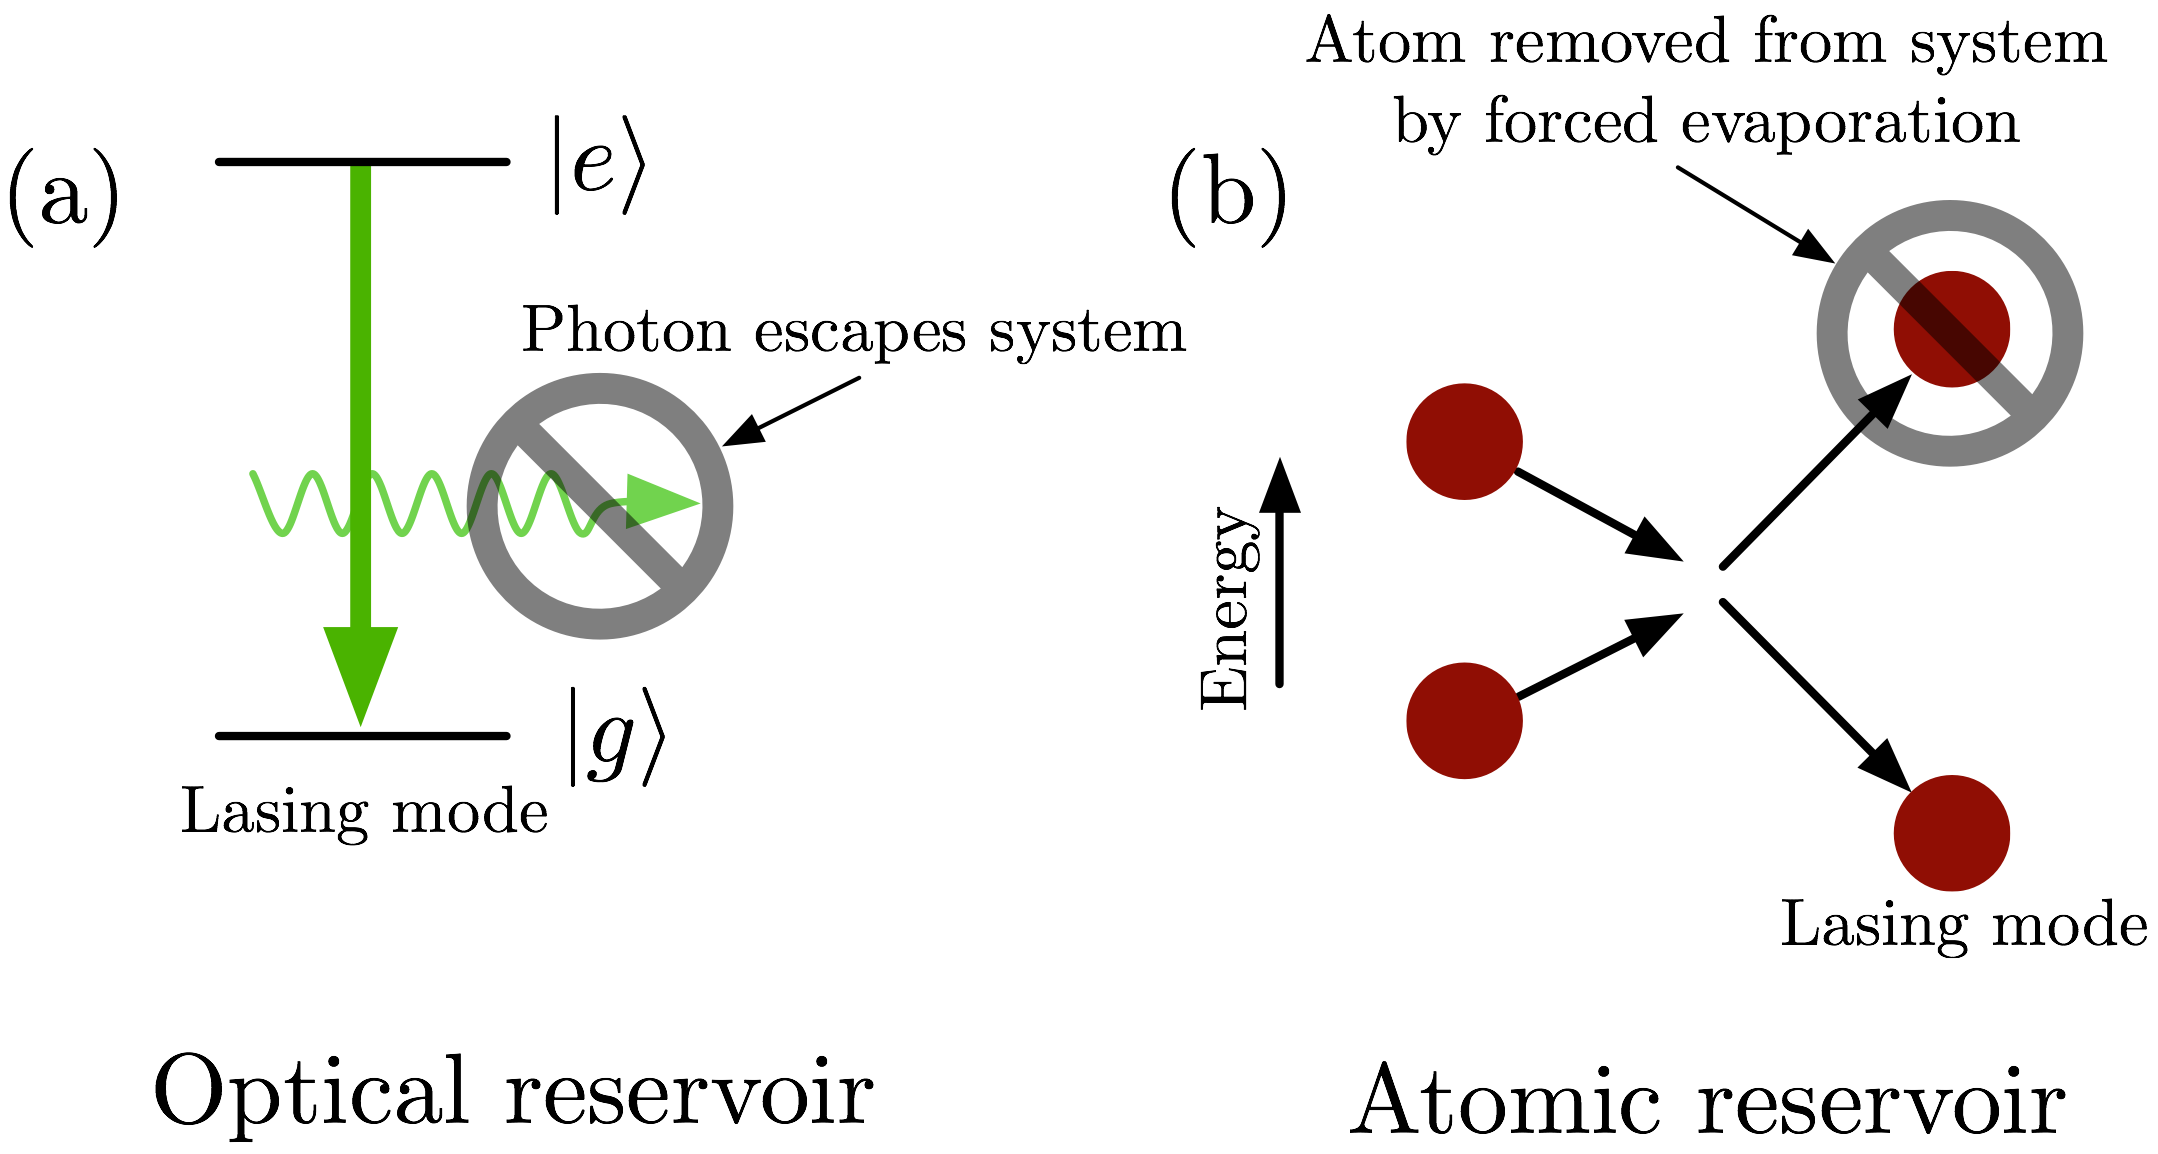
\includegraphics[width=10cm]{ReservoirChoices}
    \caption{
        \label{Introduction:ReservoirChoices}
        Classes of pumping mechanism for an atom laser as defined by the reservoir. FIXME: This is not a caption.
    }
\end{figure}

There are two choices of reservoir for the pumping mechanism of an atom laser: the empty modes of the optical field, or the empty modes of the atomic field.  Each choice corresponds to a different class of pumping mechanism.  These two classes are illustrated in \figureref{Introduction:ReservoirChoices}.  In the first, an atom in an excited internal state is brought into resonance with the lasing mode such that it can decay into the lasing mode.  It is Bose-stimulated to do so by the occupation of the atomic lasing mode.  Once the emitted photon leaves the system, this decay is irreversible.  In the second, two atoms scatter into different energy states, one goes into the lasing mode, while the other gains sufficient energy to be removed from the system (for example, due to forced evaporation, the same process used in the formation of BEC).

Single-mode operation is not simply desirable for an atom laser, it is necessary.  Due to the large interatomic interactions, multiple lasing modes in an atom laser could not operate independently.  Significant scattering would occur between the lasing modes, increasing the linewidth of both, possibly destroying any laser-like qualities in the process.  While the interatomic interactions can be `switched off' with the use of a Feschbach resonance\footnote{FIXME: Missing citation.}, the loss processes are such that higher energy modes experience \emph{less} loss than the lower modes in this case, making the atom laser unstable \citep{Haine:2002kp}.  This instability can be resolved by increasing the interatomic interactions \citep{Haine:2002kp}, adding a position-dependent loss near the edge of the lasing mode \citep{Kneer:1998fk}, and in the case of non-zero interatomic interactions, by increasing the pumping rate \citep{Robins:2001pd}.

In all of the phenomenological atom laser pumping models discussed in the previous paragraph \citep{Haine:2002kp,Kneer:1998fk,Robins:2001pd}, the gain mechanism was effectively `homogeneously broadened' in the sense that all pumping excitations could contribute equally to the gain of all modes.  This is more difficult to achieve for atom lasers than for photon lasers.  In the case of photon lasers, the dispersion relation (the expression for energy --- or equivalently, frequency --- as a function of wavenumber) for the reservoir is relatively flat by comparison to that of the lasing mode.  This is a useful property, as a greater number of pumping excitations can increase the occupation of the lasing mode if variations in the momentum difference between the pumping excitations and the lasing mode can be compensated for by the reservoir with minimal energy cost.  In the limit of a perfectly flat dispersion relation for the reservoir, any momentum difference between the pumping excitation and the lasing mode can result in gain provided only energy is conserved, and due to the finite lifetime of the pumping excitation, energy need only be conserved to within this lifetime.  As a concrete example, consider the photon laser pumping mechanism illustrated in \figureref{Introduction:4LevelOpticalLaserModel} and the atom laser pumping mechanism illustrated in \figureref{Introduction:ReservoirChoices}(a).  The fundamental difference between these two pumping mechanisms is that for the photon laser, the emitted photon goes into the lasing mode, while for the atom laser, it is the decayed atom that enters the lasing mode.  The decay process of these pumping mechanisms is illustrated in \figureref{Introduction:AtomDecay}.  If a violation of energy conservation is permitted in this process of up to $\pm \Gamma$ where $\Gamma$ is the spontaneous lifetime of the $\ket{e}$ state, excited atoms with a wider range of momenta can contribute gain to the lasing mode in the case of the photon laser than in the case of the atom laser.  Specifically, for the photon laser, the wavenumber of the excited atom in the direction parallel to the lasing mode may vary by
\begin{align*}
    \Delta k_{i,\parallel} \approx \frac{2 M \Gamma}{\hbar \abs{\vect{k}_\gamma}},
\end{align*}
where $M$ is the mass of the atom.  The wavenumber of the atom in perpendicular directions is unconstrained.  However, for the atom laser, the magnitude of the wavenumber of the excited atom may only vary by (assuming a stationary lasing mode of size $d$)
\begin{align*}
    \Delta \abs{\vect{k}_{i}} \approx \frac{2 \Gamma}{c} + \frac{\pi}{d}.
\end{align*}
For the $\lambda = \unit[633]{nm}$ lasing transition of the Helium-Neon gas laser, $\Gamma = \unit[1.4]{MHz}$ \citep[Table~13.2-1]{SalehTeich}, $M_\text{Ne} = 3.3 \times \unit[10^{-26}]{kg}$, giving $\Delta k_{i, \parallel} \sim \unit[10^8]{m\textsuperscript{-1}}$ for the photon laser and $\Delta\abs{\vect{k}_i} \sim \unit[10^{6}]{m\textsuperscript{-1}}$ for an atom laser with a lasing mode of size $d \sim \unit[10]{\micro m}$.  This difference significantly constrains the possible momentum width of the pumping excitations for the pumping mechanism to operate in the `homogeneously broadened' limit.  If the momentum width of the pumping excitations is greater than this, gain for modes other than the lasing mode will not be saturated by the lasing mode, and these other modes experiencing gain will increase the linewidth of the atom laser.  

\begin{figure}
    \centering
    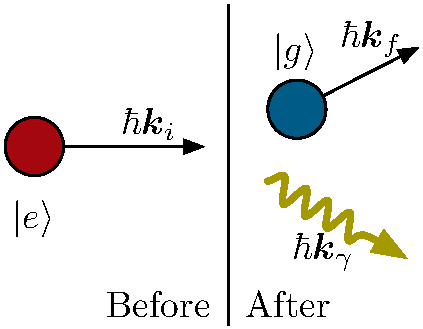
\includegraphics[width=6cm]{AtomDecay}
    \caption{
        \label{Introduction:AtomDecay}
        Excited state atom in the $\ket{e}$ state with momentum $\hbar \vect{k}_i$ decays into an atom in the ground state $\ket{g}$ with momentum $\hbar \vect{k}_f$, and a photon with momentum $\hbar \vect{k}_\gamma$.  In the photon laser pumping mechanism, the photon is in the lasing mode, while in an atom laser pumping mechanism, the decayed atom is in the lasing mode.  FIXME: This is probably not a caption.
    }
\end{figure}

In \chapterref{OpticalPumping}, a pumping mechanism for an atom laser using an optical reservoir is considered.  We attempt to solve the problem of the narrow permissible momentum width of the pumping excitations by making their momentum distribution sufficiently narrow that it can be guaranteed that every atom will be momentum-resonant with the pumping process at some point.  In \chapterref{KineticTheory}, a pumping mechanism using atomic modes as the reservoir is considered.  Although their dispersion relation cannot be considered flat with respect to that of the lasing mode atoms, it is far more so than for photons.  The difficulty with this pumping mechanism is that it is inescapable that thermal atoms will be in the vicinity of the lasing mode.  Scattering between the lasing and thermal atoms will contribute to the collisional broadening of the lasing mode.  Using a Feschbach resonance to cancel these interactions is not an option, as the pumping mechanism itself relies upon interatomic collisions.

\section{Matter wave amplification\dots}

A number of matter-wave amplification processes using the two available reservoirs have been proposed and demonstrated.  We discuss some of these in this section.  While none constitute an atom laser pumping mechanism, it would be envisaged that a pumping mechanism would be based on a process similar to those discussed. 

\subsection{\dots\ using an optical reservoir}

\subsubsection{Superradiance}
In superradiant Rayleigh scattering \cite{Dicke:1954,Rehler:1971,Inouye:1999yq,Moore:1999uq,Piovella:2001fj} off-resonant photons with momentum $\vect{p}$ are incident on a BEC, and are scattered by the condensate. When a photon is scattered into a mode with momentum $\vect{q}$, an atom absorbs the momentum difference and is scattered into the $\vect{p}-\vect{q}$ momentum state. The interference between the atoms in the $\vect{p}-\vect{q}$ momentum state and those in the BEC creates a matter-wave grating favouring further scattering of photons into the $\vect{q}$ momentum state. Similarly, the interference between the photons in the scattered $\vect{q}$ state with the incident photons creates a moving optical grating favouring the scattering of atoms from the condensate into the $\vect{p}-\vect{q}$ momentum state.  As more atoms scatter photons into the $\vect{q}$ momentum state the depth of the gratings increases, amplifying both the scattered photon and atom fields. Depending on the intensity of the photon fields, the bose-stimulation of this process can either be dominated by the photon field (optical grating) or the atomic field (matter-wave grating) \cite{Schneble:2003hb}.

%For anisotropic BECs, the maximum gain for this process occurs when photons are emitted along the long axis of the condensate, known as the endfire mode. 

Although the seed matter-wave grating for superradiant Rayleigh scattering is formed spontaneously in a random direction, phase-coherent amplification of a seed pulse can be achieved through superradiance by seeding the process with either a small matter-wave pulse in the case of stimulated Rayleigh scattering \cite{Inouye:1999ph,Kozuma:1999pi} or a weak optical laser beam in the case of collective atomic recoil lasing (CARL) \cite{Bonifacio:1994yq,Bonifacio:1994,Fallani:2005fr}.  It is interesting to note that a condensate is not necessary for superradiance; collective atomic recoil lasing was originally proposed using a cold thermal beam \cite{Bonifacio:1994yq,Bonifacio:1994}, however this process does not result in a single matter-wave grating, instead each thermal atom interferes with itself producing its own matter-wave grating. In \citeyear{Yoshikawa:2005} \citeauthor{Yoshikawa:2005} performed a similar experiment demonstrating superradiance using an ultracold gas of Rubidium atoms above the condensation temperature. One could imagine an experiment analogous to CARL in which a thermal collection of atoms could be seeded by a coherent matter-wave state stimulating phase-coherent amplification of that state in a similar manner to the amplification of a coherent optical state in CARL.

Rayleigh scattering is not the only way in which atoms can scatter light, Raman scattering is also possible whereby the atoms change internal state after scattering. Analogous to Rayleigh superradiance, Raman superradiance \cite{Schneble:2004} is also possible; in this case the matter-wave grating is not a density grating but a phase grating in the coherence between the two internal atomic states. Although both processes are possible, either process can be suppressed in an anisotropic BEC due to the different angular dependences of the emission patterns for Rayleigh and Raman scattering. By aligning the polarisation of the pump laser parallel (perpendicular) to the long axis of the condensate Rayleigh (Raman) scattering of photons can be suppressed along the long axis of the condensate, which is the mode with the most gain. By suppressing Rayleigh scattering, the difference between Rayleigh and Raman superradiance can be observed. 

In Raman superradiance, the change of the internal state of the atom after scattering suppresses higher-order processes present in Rayleigh superradiance (superradiant cascade \cite{Inouye:1999yq}) in which after scattering one photon, an atom scatters additional photons transferring it into higher momentum modes. In Raman superradiance, once an atom has scattered a photon the pump beam can become sufficiently far off one-photon resonance to significantly reduce the probability of further scattering. A group at MIT has demonstrated matter-wave amplification using Raman superradiance \cite{Schneble:2004} analogously to the earlier experiments that made use of Rayleigh superradiance. 

\subsubsection{Stuff}
Optical reservoir:
Superradiance, Rayleigh and Raman
EIT
STIRAP, Bragg diffraction?

\subsection{\dots\ using an atomic reservoir}
Evaporation to condensate?
Four-wave mixing


There are a number of processes in atom optics that display stimulated gain for matter waves.  These processes could have potential application in a pumping mechanism for an atom laser.

Issues to discuss:

Irreversibility: two choices of reservoir.
Single-mode operation: a necessity if there are non-zero interatomic interactions.
Homogeneous broadening vs inhomogeneous broadening: Due to dispersion relations, inhomogeneous broadening is basically the only possibility.  Certainly for optical pumping, and for collisional pumping...

It is important to note that the laser is a driven steady-state phenomenon, it is not necessarily similar to the BEC, which is a thermal equilibrium phenomenon.  The linewidth properties of each are not necessarily related.  This is most certainly true for the optical laser where the cavity linewidth is much larger than the laser linewidth.  

Nowhere have I given a detailed discussion of coherence.


Laser-like scheme for Atomic-Matter Waves \citep{Spreeuw:1995} --- Single mode, effective Homogeneous broadening, it works, optical pumping
An atom laser based on dark state cooling \citep{Wiseman:1995} --- Single mode, effective Homogeneous broadening, it works, optical pumping
Theory of an atom laser \citep{Holland:1996mz} --- Single mode, effective Homogeneous broadening, it works, evaporative pumping
An atom laser based on evaporative cooling \citep{Wiseman:1996} --- Single mode, effective Homogeneous broadening, it work, evaporative pumping
A model for an atom laser \citep{Olshanii:1996} --- Single mode, effective Homogeneous broadening, optical pumping
Theory of a coherent atomic-beam generator \citep{Guzman:1996} ---  Atoms trapped in an optical lattice, interacting via the dipole-dipole interaction.  This dipole-dipole interaction is mediated by the optical lattice.  The dipoles are in fact formed by the optical lattice.  Absent the ac Stark shift, the dipole-dipole interaction would be negligible.  The dipole-dipole interaction therefore occurs whenever \emph{detuned} radiation is present.  In the presence of resonant light, it may be that other effects dominate.  Their simulations are effectively single mode, effective Homogeneous broadening, dipole--dipole interaction with evaporative pumping
Cirac and Lewenstein BAR model \citep{Cirac:1996rr}
Atom laser based on Raman transitions \citep{Moy:1997} --- Single mode, effective Homogeneous broadening, optical pumping
= Generic model of an atom laser \citep{Kneer:1998fk} --- Multimode GP-based, position-independent loss, Homogeneous broadening.  Rate equation version shows threshold behaviour.  Spatially-independent loss leads to undamped excitations, spatially-dependent loss leads to a damping of these excitations.  These excitations only depend on the initial condition.
Reducing the Linewidth of an Atom Laser by Feedback \citep{Wiseman:2001zr} --- Single mode model, but demonstrates that some of the linewidth issues can be resolved by feedback
= Atom-laser dynamics \citep{Robins:2001pd} --- Multimode GP-based, 3-body loss, Homogeneous broadening.  Based on the \citep{Kneer:1998fk} model.  Includes outcoupling properly.  This symmetry-breaking term changes the lowest excited mode form the breathing mode to the sloshing (Kohn \citep{Dalfovo:1999ly}) mode. 
Continuous optical loading of a Bose-Einstein condensate \citep{Santos:2001ve} --- Few mode model, Homogeneous broadening.  Optical pumping.
More feedback reducing the linewidth \citep{Thomsen:2002xc}.
= Stability of Continuous Pumped Atom Lasers \citep{Haine:2002kp} --- Locally-saturable GP-based model.  Position-independent one- and two-body loss, Raman outcoupling.  Although the parameters were not chosen to operate in the locally-saturated mode.  Instead it was globally-saturated (effectively Homogeneously broadened).  The characteristic diffusion timescale was $\sim \unit[10^{-6}]{s}$.  Hence the problem.  Regardless, in the zero-interaction limit, it is found that higher-energy modes are more spread out and therefore suffer lower two-body loss.  This leads to an instability.  Note that if this was modelled with proper locally-saturable pumping mechanism, not only would the higher modes suffer less loss, they would also experience greater gain, as they can source gain from a larger area.  In the presence of interactions, it may be hoped that there will be suppression of excitations as their mode shape will have changed.  It was demonstrated that increasing the scattering length suppressed excitation of the higher modes.


Saturation also contributes to the single-mode operation of optical lasers.  


The pumping mechanism for an optical laser not only permits the continuous operation of the laser, but it can also narrow the linewidth of the laser in a process known as \emph{gain-narrowing}.  

Inhomogeneously-broadened gain media also show gain narrowing.

For homogeneously-broadened gain media, this also prevents multimode operation.

Gain-narrowing is caused by the saturation of the pumping process, and although the pumping process does not need to be saturable for the output of the laser to be coherent (or to have any other properties typically associated with a laser \citep{Wiseman:1997ba}), it is a property that increases the utility of atom lasers for 

: The linewidth of the optical cavity is related to the Fourier limit.


The pumping mechanism for an optical laser not only permits the continuous operation of the laser, but it can also narrow the linewidth of the laser in a process known as \emph{gain-narrowing}.  Gain-narrowing is caused by the saturation of the pumping process, and although a pumping process does not need to be saturable for the output of a laser to be coherent (or to have any other properties typically associated with a laser \citep{Wiseman:1997ba}), it is a useful property that would be convenient to have for atom lasers.  In particular, it is desirable that an atom laser pumping mechanism be uniformly saturable in the sense that stuff.



Without a pumping mechanism, an optical laser is simply a leaky cavity emitting an exponentially decreasing amount of light with the same linewidth as the optical resonator.  The pumping mechanism for an optical laser not only permits the continuous operation of the laser, but it can also narrow the linewidth of the laser 

also narrows the linewidth of the laser below the bare cavity linewidth in a process known as \emph{gain-narrowing}.  Gain-narrowing is caused by the saturation of the pumping process, and although a pumping process does not need to be saturable for the output of a laser to be coherent (or to have any other properties typically associated with a laser \cite{Wiseman:1997ba}), it is a useful property that would be convenient to have for atom lasers.

The difference is between homogeneous broadening (gain-narrowing) and inhomogeneous broadening.  In the case of homogeneous broadening, all of the excitations of the pumping process access all of the potential optical modes for pumping. In inhomogeneous broadening, each excitation can only access a range of the potential optical modes; one dominant mode may saturate pumping excitations that may access that mode, but there will exist other pumping modes which are not saturated, and these may excite different modes.  This is a problem that is observed in certain atom laser pumping mechanism with a locally-saturable pumping reservoir.  \citep{SalehTeich}.



Here we discuss pumping and matter-wave amplification.

Contemporary atom optics experiments operate in pulsed mode, and consistent with the analogy with a pulsed optical laser, these experiments are frequently limited by the linewidth (velocity-spread) of the atomic pulse produced. The present limit on this linewidth is proportional to the inverse of the outcoupling time for pulsed atom lasers \cite{Johnsson:2007}.  This limit can be made arbitrarily small (until the energy uncertainty in the BEC due to s-wave scattering becomes significant \cite{Johnsson:2007a}) at the expense of an arbitrarily small atom flux.  Practically, however, this trade-off cannot be made because the signal-to-noise ratio for these experiments depends critically on the atomic flux.  Alternatively, a continuous atom laser, in analogy to a continuous optical laser could operate for an arbitrary period of time independent of the atomic flux, hence reducing the linewidth of the atom laser until the s-wave scattering limit \cite{Johnsson:2007a} or a limit analogous to the Schawlow-Townes limit for optical lasers \cite{Schawlow:1958} was reached.


Without a pumping mechanism, an optical laser is simply a leaky cavity emitting an exponentially decaying amount of light with the same linewidth as the optical resonator.  The pumping mechanism for an optical laser not only permits the continuous operation of the laser, but it also narrows the linewidth of the laser below the bare cavity linewidth in a process known as \emph{gain-narrowing}. Gain-narrowing is caused by the saturation of the pumping process, and although a pumping process does not need to be saturable for the output of a laser to be coherent (or to have any other properties typically associated with a laser \cite{Wiseman:1997ba}), it is a useful property that would be convenient to have for atom lasers.


The other necessary property of a pumping mechanism is that the coupling process gives rise to a biased transfer of bosons from the pumping mode to the lasing mode.  In a generic laser pumping process (see \figureref{fig:PumpingMechanism}), one or two initial bosons are coupled with a Bose-enhanced coupling rate to a state with an additional boson in the lasing mode, and a secondary boson in a different state.  To prevent the possibility of this process removing bosons from the lasing mode, the state occupied by the secondary boson must be initially unpopulated, as if there were any population in this state it would be possible for the pumping process shown in \figureref{fig:PumpingMechanism} to run backwards.  Although this requirement will prevent any bosons being removed from the lasing mode, it does not guarantee that once a boson has been transferred to the lasing mode that it will not be removed again due to coupling back to the initial state.  To ensure that this does not occur, the secondary boson in the laser pumping process must irreversibly change state such that it can no longer interact in the pumping process, this is usually achieved by changing the internal state of the secondary boson or by removing it from the interaction region.  In an optical laser the initial boson is an atom in an excited state and it is coupled to a state where the atom has de-excited by emitting a photon into the lasing mode. To prevent the de-excited atom re-absorbing a lasing-mode photon and reversing the pumping process, this de-excited atom needs to rapidly change internal states. In a four-level laser pumping scheme this is achieved by ensuring that the atom in the de-excited state has a rapid, irreversible decay down to a lower state from which it can later be re-excited by the pump; in a three-level laser pumping scheme the de-excited atom is directly and irreversibly pumped to a highly-excited state.

\section{Pumping and Matter-wave amplification}

\section{Thesis overview}

\hrule

\section{Atom lasers}
\label{Introduction:AtomLaser}


\section{Pumping and (atom) lasers}
\label{Introduction:Pumping}

FIXME: This content to go in the introduction.

A brief overview of what gives a laser its properties. Refer to Wiseman's paper~\citep{Wiseman:1997ba} and compare the optical and atom lasers. Alternatives for the irreversibility / source are discussed in \chapterref{OpticalPumping,KineticTheory}.

There are two fundamental reasons making the pumping of an atom laser harder than pumping an optical laser is that the dispersion relation for potential reservoirs is not flat by comparison to the dispersion relation for atoms.  For an optical laser in the homogeneous broadening limit, \emph{all} atoms in the sample can contribute to gain.  Fundamentally this is because independent of what momentum the atom might have, it can still be stimulated to emit a photon into the lasing mode as the decay rates of the excited and/or ground atomic states are greater than any possible energy detuning in this process.  The second fundamental issue affecting atom lasers is that atom number is conserved.  It is therefore inescapable that there will be atoms in a (potentially) non-condensed source mode in the vicinity of the lasing mode.  Unless a Feschbach resonance is used to set the scattering-length of atomic interactions to zero, the atoms in the source mode will disrupt the phase stability of the lasing mode.

In \chapterref{OpticalPumping}, we attempt to solve the first problem by making the momentum distribution of source atoms sufficiently narrow that it can be guaranteed that every atom will be momentum-resonant with the pumping process at some point.  In \chapterref{KineticTheory}, we use atomic modes as the reservoir.  Although their dispersion relation cannot be flat with respect to that of the atoms in the source mode, it is at least far more comparable than that of light (which is used in \chapterref{OpticalPumping}).

Ideally we should pump an atom laser using something with a flat dispersion relation.  One possibility that comes to mind is the phonon.  However it is necessary that the reservoir is essentially a pure vacuum.  Phonons produced in a condensate cannot escape the system unless the system is in contact with other atoms.  If these other atoms are thermal, than it will have its own phonons which will propagate into the condensate.  If the condensate is not in physical contact with anything, then the phonons cannot leave the system: there is no evaporation process for phonons.

Stolen from \citep{Ballagh:2000oq}:
Despite the parallels with optical laser theory, the fundamental differences between photons and atoms remain important. They arise principally because atoms have rest mass, and because they interact with each other. Unlike photons, atoms cannot be created or destroyed, rather they are transferred into the laser mode from some other mode. The interactions produce phase dynamics, which degrades the coherence of the atom laser, and self repulsion which spreads the output beam and limits the possible focussing. Even when these interactions are neglected, atoms have dispersive propagation in vacuum.
